\section{Introduction}

%% 
%% Leave first page empty
\thispagestyle{empty}

Video communication is rapidly changing, the dramatical increase of Internet communication between people is forcing technology to support mobile and real-time video experiences in different ways. Applications such as {\it Vime} and {\it Skype} provide media and real-time communication over the Internet. 

Technology and media are changing the way people interact with each other, communication over the internet is encouraging users to interact, talk and see content in a cost-effective and reliable way. Business structure and innovation is rapidly changing thank to the existence of reliable, low cost and simple platforms for real-time communication.

This way of communication is adding new features to services that have never been available before, they are now able to have high-engagement communication, where richer, more intimate communication is possible~\cite{futureRTC}. At the same time, this is changing traditions and habits of communication between people and transforming personal relationships~\cite{socialrelationships}. Distances are now shorter, bringing individuals and groups together around the world, allowing people to connect with friends and meet new people in different ways such as gaming or using social networks.

Furthermore, it also helps businesses to have lightweight communication alternatives that will increase their efficiency besides the size of the company. 

Real-time communication is encouraging front end designers designers and device developers to turn their products into multi-functional and interoperable communication devices.

Video has been available in the World Wide Web (WWW)\nomenclature{WWW}{World Wide Web} since the 1990s, it has evolved to be less CPU consuming and has adapted to the new link rates (e.g DSL, 3G or EDGE) while affordable digital and video cameras have become integral parts in nowadays computers. Those two enablers along with the increased demand for richer applications with easy integration for the WWW are some of the reasons behind Real Time Communications for the Web (WebRTC)\nomenclature{WebRTC}{Real Time Communications for the Web}.

WebRTC is a suite of tools that enable human communications via voice and audio where Real Time Communication (RTC)\nomenclature{RTC}{Real Time Communication} should be as natural in a web application as browsing images or visiting websites instead of requiring extra software to be installed. With this simple approach, WebRTC aims to transform something that has been traditionally complex and expensive into an open application that can be used by everybody, enabling this RTC technology in all existing web applications and giving the developers the ability to innovate and allow rich user interaction in their products using an standardized and free technology.

Many web services already use RTC technology to allow communication (e.g., Google Hangouts and Adobe RTMFP) but most of them require the user to download native apps or plugins to make it work. With WebRTC, real-time communications between users should be transparent for them, since downloading, installing and using plugins can be complex and tedious. On the other side, the usage of plugins is also complicated from the development point of view and restricts the ability of developers to come out with great features that can enrich the communication between people.

WebRTC project major guidelines are based on working Application Programming Interfaces (APIs) \nomenclature{API}{Application Programming Interface} that are free to use and openly standardized.


%The need of a new way to communicate between two points of the planet is a problem that many different technologies have tried to approach. Systems such Skype or VoIP are not able to cope the needs of the new generations of developers and users that everyday require a more integrated way of communication with the World Wide Web (WWW)\nomenclature{WWW}{World Wide Web}. 
%
%Besides this, the amount of data transferred during the last years and the prevision for the future allocates a new scenario where non-centralized systems such as P2P are required as data bandwidth grows and systems need to become more scalable. Nowadays, networks are still manly content-centric, meaning that data is provided from a source to a client in a triangle scheme, clients upload data to central servers and this data is transferred to the endpoint. This architecture has been provided since long time as reliable and scalable, but with the appearance of powerful applications and Video On Demand (VOD) scalability is becoming an issue.
%
%Those circumstances lead to a whole new world of real-time browser based applications which require also a new framework to work with. Ranging from online videoconferencing to real-time data applications, for this purpose few attempts were made in the past being highly reliable on specific hardware and custom-built no-compatible systems. Those proposals were not accessible to normal users that could not afford to adapt the requirements. 
%
%All previous concepts are now possible thanks to the increase of the average performance in every computer nowadays, this situation is helping to build more complex browsers that are able to perform many different tasks that enhance web browsing to a different level. Having a browser to handle OpenGL style of applications is now possible thank to the new  HyperText Markup Language version 5 (HTML5) standard. Multimedia abilities are also able to be reproduced on those browsers and webcam media shown as HTML is now a reality. Even dough, there is still an important issue that must be addressed: there is no common standardized protocol that allows developers to do this. Web Real-Time Communication (WebRTC) effort to approach this problem is to build a simple and standard solution for peer-to-peer browser communication in the HTML5 environment~\cite{alvestrandOverview2012} .
%
%Internet bandwidth capabilities helped to take the decision to start integrating peer-to-peer solutions in browsed based applications, this is due the year-by-year increase of user bandwidth connectivity during the last 10 years. Actual latency in the network is low enough to allow real-time applications to work resiliently in the browser. The amount of users being able to transfer at high speed has increased during last years (Figure~\ref{fig:bwWorldAvg}), about 39\% of users are able to download at speeds greater than 4Mbps being this a very good average speed for multimedia content~\cite{akamaiq2}.
%
%\begin{figure}[h]
%  \centering
%    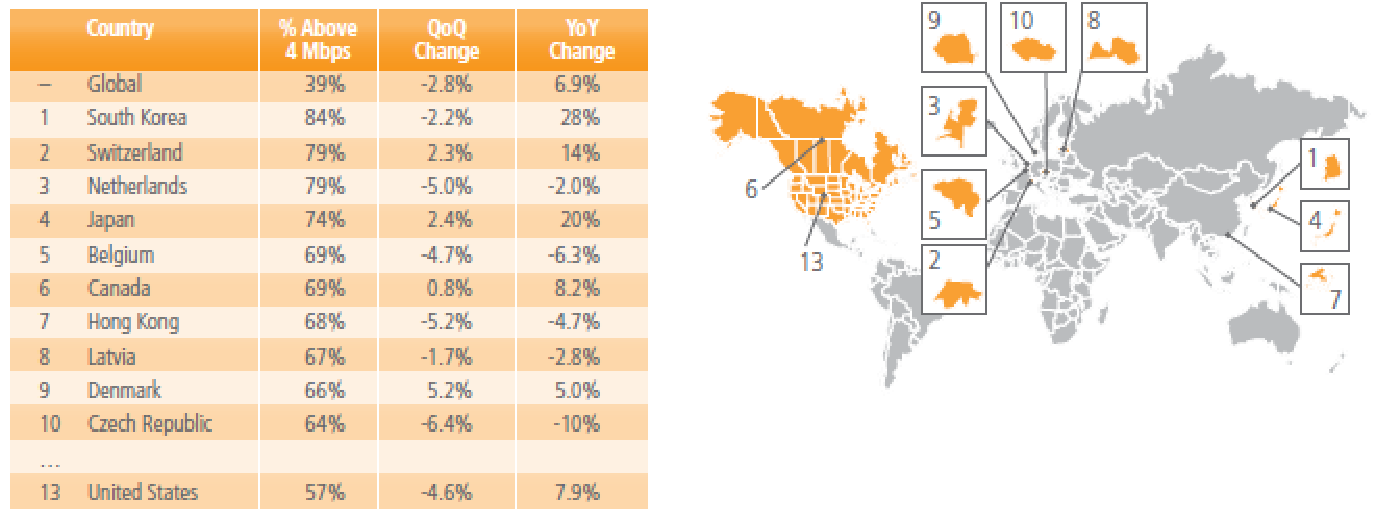
\includegraphics[width=1\textwidth]{./figures/internetstats.pdf}
%      \caption[Broadband over 4Mbps connectivity statistics]{Broadband connectivity statistics about the speeds over 4Mbps around the globe.}
%	\label{fig:bwWorldAvg}
%\end{figure}
%
%Regarding the specs on the client side, recent surveys and statistics taken by the game manufacturer Steam prove that more than  61\% of machines are carrying 1 to 4 gigabytes of RAM and nearly 90\% of computers handle 2 to 4 core CPU with a 64 bit OS~\cite{steamStats}, this environment can easily handle media enhanced applications that require high performance for media encoding. WebRTC concept rests over multiple layers having the browser as an underlying application, a traditional browser allocates a lot of resources for running being the performance of the machine a bottleneck in some cases.
%
%Traditionally, WebRTC concept approaches rely on the usage of plug-ins or other separate software components that make the system run smoother by avoiding one layer of processing (browser) but being non-standard and not cross-compatible, one of the most import ant concepts when designing applications nowadays. This approach has a new alternative with the arrival of the new HTML5 where WebRTC is integrated as one of the new Application Programming Interfaces (APIs) available alongside other many different interesting capabilities.

\subsection{Background}

WebRTC is an effort to bring real-time communication APIs to JavaScript developers, allowing them to build RTC functionalities into web applications that enable different features, such as video calling platforms over the web. 

Web application APIs are defined in the HyperText Markup Language (HTML) \nomenclature{HTML}{HyperText Markup Language} version 5 and help developers to add features to their web applications with minimal effort using JavaScript functions. APIs can be defined as a collection of methods and callbacks that help developers to access available technologies in the browser, they are used in web development to access the full potential of browsers and compute some part of the dynamic web applications on the client side.

WebRTC APIs works by combining two different technologies, HTML and JavaScript, HTML is the de facto markup format for serving web applications and JavaScript is becoming the most popular scripting system for web clients to allow users to dynamically interact with the web application. 

The actual version of WebRTC is formed between different API that integrate with each other to provide flexible RTC in the browser. However, the final goal is to allow developers to create plugin-free real-time web applications that are cross compatible with different browser vendors and operating systems.

The flexibly of WebRTC allow many uses of RTC thus foreseeing many new topologies that will emerge. Developing RTC technologies over the Internet has been always closely related to the topology distribution of the nodes that are being connected, performance issues in different topologies usually restrict the amount of nodes available for the session. From the simple point-to-point topology to the mesh composition, choosing the right option for each application is very important to deliver a great user experience.

%This part of history can be removed if needed
\subsection{History}

WebRTC API is being drafted by the World Wide Web Consortium (W3C) \nomenclature{W3C}{World Wide Web Consortium} alongside with the Internet Engineering Task Force (IETF) \nomenclature{IETF}{Internet Engineering Task Force}. This API has been iterated through different versions to increase its usability thanks to the feedback given by web developers.

The first W3C announcement of WebRTC was done in a working group in May 2011~\cite{webrtcW3cgroup}, and the official mailing list started in April 2011~\cite{welcomeW3C}. During the first stage of discussion, the main goal was to define a public draft for the version 1 of the API implementation and a timeline with the goal to release the first final version of WebRTC. The W3C public draft of WebRTC was published on 27th of October 2011~\cite{originalW3Cdraft}. This first W3C draft only specifies how to send media (audio and video) over the network to other peers, it defined the way browsers would be able to access media devices without the use of any plugin or external software.

WebRTC project got involved with the IETF in May 2011~\cite{webrtcIETFgroup}. The initial milestones of the IETF initially marked December 2011 as the deadline to provide the information and elements required for the W3C to design the first version of the API. On the other side, the main goals of the IETF working group are the definition of the communication model, session management, security, NAT traversal solution, media formats, codec agreement and data transport~\cite{webrtcIETFcharter}. In June 2011 Google publicly released the source code of their WebRTC API implementation~\cite{haraldpublicWebRTC}. 

WebRTC APIs are integrated within the browser and accessible using JavaScript in conjunction with the Document Object Model (DOM) interfaces. Some of the APIs that have been developed for WebRTC are not part of the HTML5 W3C specification but are included into the Web HyperText Application Technology Working Group (WHATWG) \nomenclature{WHATWG}{Web HyperText Application Technology Working Group} HTML specification.

% This HTML version includes different API's and JavaScript function that help the developer to easily introduce new features into their already existing WWW applications. The initial HTML version (2.0) was published in November 1995 with the only goal of delivering static content from the server to client browser~\cite{html2IETF}. HTML became de de facto format for serving web information. 
%
%HTML is written in tag formatting to identify different elements. Those tags are then interpreted by the browser to show the different data content served by the server. During the evolution of the WWW different new features have been added to the HTML standard and new versions where published, things like JavaScript and Style Sheets increase the flexibility and features of the WWW content enhancing the final user experience.

%Due to the need to extend the features of the already existing HTML4 standard, a new version was proposed in 2004 by the Mozilla Foundation and Opera Software~\cite{initialHTML5proposition}. This new proposition focused in new developing technologies that could be backwards compatible with the already existing browsers, the idea didn't make a success and was tier apart until January 2008 when the first Public Working Draft was published by the Web HyperText Application Technology Working Group (WHATWG) in the W3C~\cite{firstHTML5draft}.

%HTML5 proposal had a greater reliance in modularity in order to move forward faster, this meant that some specs that were included in the initial draft moved to different working groups in the W3C~\cite{firstHTML5draft}. Those technologies defined in HTML5 are now in separate specifications, one of them being WebRTC. 

\subsection{Challenges}

WebRTC is a suite of protocols that share the available device resources with many other applications. Due to the little experience in WebRTC environments sharing the available resources, we find some lack of documentation or previous literature regarding congestion analysis compared with other technologies. During the development of the thesis we focus in the technical challenges of the protocol.

The aim to test and help to develop new protocols such as WebRTC is unfortunately accompanied by a lack of information that may affect some of the statements made in this thesis that could change in future versions of WebRTC, even dough it should not affect the overall conclusions.

Considering the fact that WebRTC is still being developed at the moment of writing this thesis, some of the statements made here might be different in the upcoming versions of WebRTC, meaning that some of the analyzed issues could have been solved.

General WebRTC challenges are related to technical problems. Firstly, congestion mechanisms for RTC have always been complicated to implement due to the need of a fast response against path disturbances and link conditions. During the course of this thesis we might find limitations in WebRTC when having constrained links.

Network Address Translation (NAT) \nomenclature{NAT}{Network Address Translation} may also arise as a problem, succeeding when setting up a communication path through restrictive environments is crucial in RTC protocols.

On the other side, we will also study the available topologies for RTC and which one of them fit in a WebRTC environment, trying to understand the limits of the protocol in different scenarios and topologies. All the structures that can be implemented using WebRTC might have some restrictions in performance and user experience that we need to study and understand, those limitations are important when designing WebRTC applications.

\subsection{Contribution}

Investigate how WebRTC performs in a real environment trying to evaluate the best way to set multiple peer connections that handle media in different network topologies. 

Measure the performance of WebRTC in a real environment, identifying bottlenecks related to encoding/decoding, media establishment or connection maintenance. All this should be performed in real-time over a browser by using the already existing WebRTC API. By using metrics related to RTC protocols we expect to understand the way WebRTC performs when handling in different environments.

\subsection{Goals}

WebRTC uses and adapts some existing technologies for real-time communication. This thesis focuses in studying:

\begin{itemize}
	\item WebRTC performance in different topologies and environments using real sources of video and audio that are encoded with the codec provided by the browser.
	
	\item Usage of WebRTC to build a real application that can be used by users proving that the API is ready to be deployed as well as it is a good approach for the developer needs when building real-time applications over the web. This is done in conjunction with other new APIs and technologies introduced with HTML5.
	
	\item Testing of different WebRTC topologies with different network constraints to observe the response of the actual existing API.
\end{itemize}

The final conclusion covers an overall analysis and usage experience of WebRTC, providing some valuable feedback for further modifications on the existing API.

\subsection{Structure}

This thesis is structured as follows: 

\begin{enumerate}
\item Introduction of real-time communication
\item Description of different protocols used for real-time communication and the APIs that are built within WebRTC
\item Definition of different possible topologies used for real-time communication
\item Analysis of the required metrics used to evaluate WebRTC performance
\item Environment setup used to evaluate WebRTC 
\item Result and analysis of the different scenarios that can be given in WebRTC applications
\item Conclusions of the thesis
\end{enumerate}
